\section{Opis i założenia projektu}
    Celem projektu jest zaprojektowanie oraz zbudowanie systemu analizatora stanów logicznych.
    System analizatora składa się z 2 części:
    \begin{itemize}
        \item Układu analizatora - dedykowane PCB zawierające min. mikrokontroler
        Raspberry Pi Pico W, przetwornik ADC, układ filtracji sygnału analogowego (LPF)
        oraz interfejs wejściowy wraz z zabezpieczeniami chroniącymi układ przed przypadkowymi
        pomyłkami użytkownika.
        \item Aplikacji komputerowej - interfejs użytkownika odpowiadający za intuicyjną
        komunikację między użytkownikiem a urządzeniem. 
        % W celu zapewnienia responsywności, aplikacja powinna dzielić wyświetlanie oraz przetwarzanie danych na oddzielne wątki.
    \end{itemize}

\subsection{Przegląd dostępnych rozwiązań}
    \begin{enumerate}
        \item Analog Discovery 3 (AD3).
        \newline AD3 to przenośne, wielofunkcyjne narzędzie pomiarowe wyposażone min.:
        oscyloskop, generator sygnałów, analizator logiczny oraz multimetr.
        \begin{figure}[H]
        \centering
        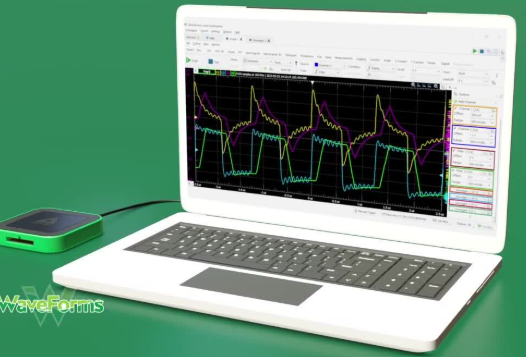
\includegraphics[width=0.6\textwidth]{AD3.png}
        \caption{Analog Discovery 3}
        \label{fig:AD3}
    \end{figure}

    AD3 charakteryzuje się parametrami takimi jak:
    \begin{enumerate}[label=\arabic*.]
        \item Oscyloskop: rozdzielczość ADC 14 bitów, liczba kanałów 2, prędkość próbkowania do $200 MSap/s$
        \item Analizator Stanów logicznych: liczba kanałów 16, prędkość próbkowania do $200 MSap/s$
        \item Generator: rozdzielczość DAC 14 bitów, maksymalna częstotliwość (dla $sin(x)$) do 20 MHz, 
        liczba kanałów: 2 analogowe
        \item Cena ~1900zł (DigiKey)
    \end{enumerate}

    \item PicoScope 3404D. 
    \newline PicoScope to przenośny oscyloskop USB z 4 kanałami analogowymi i
    16 kanałami cyfrowymi. Urządzenie posiada dodatkowo wbudowany generator
    sygnałów oraz zaawansowane funkcje analizy protokołów i sygnałów.
        \begin{figure}[H]
        \centering
        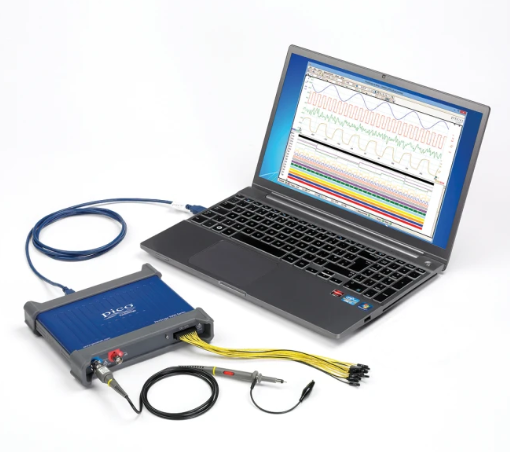
\includegraphics[width=0.6\textwidth]{PicoScope.png}
        \caption{PicoScope 3404D}
        \label{fig:PicoScope}
    \end{figure}

    PicoScope 3404D charakteryzuje się parametrami takimi jak:
    \begin{enumerate}[label=\arabic*.]
        \item Oscyloskop 14-bit rozdzielczości, 4 kanały, do $1 GSap/s$ próbkowania (do $10 GSap/s$ z trybem ETS)
        \item Analizator stanów logicznych: 16 kanałów, prędkość próbkowania: do $100 MSap/s$ próbkowania
        \item Generator 14-bit rozdzielczości DAC, maksymalna częstotliwość (dla $sin(x)$) do $20 MHz$ 
        \item Cena: $6500 zł$ (Farnell)
    \end{enumerate}

    \end{enumerate}



\subsection{Założenia sprzętowe}
    \begin{enumerate}
        \item Analizator stanów logicznych, jako układ pomiarowy nie powinien obciążać prądowo
        urządzenia badanego, dlatego system będzie pracował w trybie
        wysokiej impedancji wejściowej.
        \item Podstawowe parametry układu to:
        \begin{itemize}
            \item Wysoka szybkość próbkowania sygnałów cyfrowych.
            \item Odpowiednia rozdzielczość pomiarowego toru analogowego.
            \item Stabilna praca.
        \end{itemize}
        \item Maksymalna częstotliwość próbkowania sygnałów cyfrowych powinna wynosić $f_{\text{sample}} = 50MHz$.
    \end{enumerate}

\subsection{Założenia oprogramowania}
    \begin{enumerate}
        \item Aplikacja komputerowa powinna stanowić wygodny oraz intuicyjny interfejs
        między użytkownikiem a urządzeniem.
        \item Oprogramowanie mikrokontrolera w maksymalnym stopniu powinno opierać się na
        zasobach sprzętowych układu takich jak DMA, timery, akceleratory IO (PIO) itp. .
    \end{enumerate}

\subsection{Podział obowiązków}
    \textbf{Łukasz Przystupa}
    \begin{enumerate}
        \item Stworzenie aplikacji komputerowej.
        \item Zaprojektowanie niskopoziomowego systemu próbkującego sekcji cyfrowej opartego o PIO wbudowany w Raspberry PI PICO.
        \item Konfiguracja bardzo szybkiej i stabilnej komunikacji szeregowej między
        komputerem użytkownika a PicoProbe z wykorzystaniem interfejsu USB.
    \end{enumerate}

    \textbf{Krzysztof Płonka}
    \begin{enumerate}
        \item Napisanie biblioteki do obsługi czujnika ADC ADS1115.
        \item Zapewnienie komunikacji bezprzewodowej między Pi Pico a aplikacją graficzną.
        \item Dodanie funkcjonalności obserwacji sygnałów analogowych
        (biblioteka gtk live-chart, integracja z SigRok lub biblioteka CAIRO)\footnote{Opcjonalnie.}.\\ 
    \end{enumerate}

    \textbf{Paweł Olbrych}
    \begin{enumerate}
        \item Projekt PCB.
        \item Dobór elementów.
        \item Zaprojektowanie min.: interfejsu wejściowego układu analizatora stanów,
        interfejsu wejściowego przetworników ADC, układu filtracji oraz polaryzacji zasilania oraz
        mniejszych podobwodów pomocniczych. 
    \end{enumerate}
    